%!TEX root = these.tex

\chapter{Real-Time Streaming Communication with Optical Codes}

This chapter represents a reformatted version of a paper published in 2016 in IEEE Access, v.4, p. 284-298 by K. Xie, S. Gaboury and S. Hallé.

\section*{Abstract}
Optical codes have long been used to carry small amounts of static data, such as URLs, IDs or other short binary sequences. In this chapter, we experiment on the use of sequences of optical codes to form a one-way communication channel. In this context, a sender is made of a surface displaying rapidly changing codes, which are picked up by a receiver's camera and converted back into a binary data stream. After presenting experimental results seeking the combination of frame rate, code size and error correction level maximizing effective bandwidth, we describe the implementation of a robust communication protocol designed specifically for lossy, simplex, and low-bandwidth data links. Our findings indicates that such a protocol is sufficient for carrying at least voice-quality audio in realtime.

%% -----------------------
%% Section: intro
%% -----------------------
\section{Introduction}\label{sec:qr:intro} %% {{{

Wireless communication is a technology that allows two or more peers to communicate without electric cables or conductors \citep{tse2005fundamentals}. While the majority of wireless communication technologies uses radio waves as their transmission medium, a few others use light, especially in situations where radio technology is difficult to apply. Optical communication in itself reaches back to the use of flags, smoke signals and signal lamps to communicate information between two points with the use of a specific code~\citep{burns2004}.

Recently, a simple form of optical communication, called \emph{Quick Response Code} (QR code) \citep{qrcode-about}, emerged as a refinement over the existing technology of one-dimensional barcodes. Owing to their accuracy and their considerable capacity, QR codes have been used in many areas; applications for handling such codes have also been ported to a variety of devices, including desktop computers, smartphones, and even television sets.

However, so far QR codes have been used for the transmission of \emph{static} data. Generally a code is printed on a physical medium, such as a sheet of paper, and is read by an optical device (typically a camera) for decoding at a later time. In this chapter, we explore the idea of extending QR codes and turn them into a dynamic, one-way communication channel. In such a channel, a stream of data is transmitted through a \emph{sequence} of codes; typically, these codes are continuously generated and displayed on one device, and simultaneously captured and decoded by another, hence performing the same task as other kinds of communication technologies.

After briefly describing in Section~\ref{sec:qr:reading} the basics of QR codes and other wireless communication technologies, we shift our focus in Section~\ref{sec:qr:qrcode} to the principle of raw QR code communication. In particular, we attempt to find the intrinsic limits of such a communication channel, by analyzing the influence of a variety of factors, such as code density, number of codes displayed per second, etc. The results of an experimental benchmark considering more than a hundred different combinations of parameters allow us to extract optimal conditions that minimize the rate of error in decoding the images, while maximizing the amount of data that can be transmitted per unit of time.

%The code decoding depends on the quality and the complexity of the captured image. If the image is broken or blurred, it will be difficult to decode. And the algorithms of image recognition may have the probability of failure\cite{adel2006}. Therefore, at first, we did a benchmark with combinations of the parameters, such as the camera configuration, the frame rate, and the data size in one code. According to the benchmark result, we selected an optimal combination for our second step.

These first results indicate that QR code streams can indeed be used as a simple, one-way channel, but that error-free communication and high-bandwidth are more or less impossible. Therefore, as a second step, we design a protocol suitable for the specific nature of QR code communication. This protocol, called BufferTannen, is described in Section~\ref{sec:qr:protocol}. It is able to encapsulate raw data, provides various signaling capabilities, can represent semi-structured data (such as JSON) in a compact binary form, and supports data framing/deframing and streaming.

A second experiment reveals the robustness of this transmission scheme: using our specially designed protocol, the communication channel created by a person pointing a smartphone at arm's length towards a flickering QR display produces sufficient bandwidth to transmit voice-quality audio in real time. Section~\ref{sec:qr:experiments} presents the environment and the results of the experiments of this second step. We also show how a piece of data, cut into multiple codes with the use of BufferTannen, can be reconstructed automatically by a user hovering his camera over a sheet of such printed codes in no particular order.

This work was originally motivated by a practical application in the field of runtime verification. In past research, we suggested and informally experimented the use of optical codes as a form of loosely coupled communication between a software system and an external monitor receiving events produced by that system \citep{DBLP_conf/rv/LavoieLVGH14}. In this context, communication through optical means ensured a complete isolation between the system and its monitor.

Although the use of sequences of QR codes has been informally suggested in the past, to the best of our knowledge, our study is the first systematical investigation of the potential of QR codes to send streams of data in real time. %Because QR codes are basically images, besides being displayed on the screen, they can be also distributed in other ways, for example, they can be printed on the papers or other printable surfaces. 

The solution we propose provides a method for distributing streaming data without dedicated communication devices. The only required devices are a common camera (such as a webcam or the camera on any cellphone) and a small flat surface to display the sequential QR codes ---for example, a computer, television or smartphone screen, or even a sheet of paper.

%% }}} --- Section

%% -----------------------
%% Section: comment on lit les codes QR
%% -----------------------
\section{Wireless Communications}\label{sec:qr:reading} %% {{{

This section recalls a few common wireless communication technologies. Despite their popularity and performance, each has its own limitations and application scenarios. %, which leads to our problematic: find another communicating solution and prove its feasibility.

\subsection{Radio Waves}

The first obvious means of wireless communication is through the use of radio waves, and is best exemplified through WiFi \citep{Comer:2008:CNI:1816918}, used for local area wireless networking. Its variants are based on the IEEE 802.11 family of standards, and support both centralized (routing) and decentralized (\textit{ad hoc}) networking. Table \ref{tab:qr:wifi-protocol} shows popular 802.11 standards and part of their specifications.

\begin{table}[ht]
\begin{center}
\begin{tabular}{|l|l|l|l|}
\hline
Protocol &	Frequency & 	Max. physical data rate &	Indoor range\\
\hline
802.11a &	5 GHz &	54 Mbps &	35 m \\
\hline
802.11b &	2.4 GHz &	11 Mbps &	35 m\\
\hline
802.11g &	2.4 GHz &	54 Mbps &	38 m\\
\hline
802.11n &	2.4/5 GHz &	150 Mbps &	70 m\\
\hline
802.11ac &	5 GHz &	866.7 Mbps & 35 m\\
\hline
\end{tabular}
\caption{A summary of WiFi protocols\citep{theng2008ubiquitous,perahia2013next}}
\label{tab:qr:wifi-protocol}
\end{center}
\end{table}

A second contender in this family is Bluetooth \citep{Comer:2008:CNI:1816918}, which is used for short-range and generally point-to-point communication between devices. Its range varies from about 1 to 100 meters depending on the class of power. Table \ref{tab:qr:bluetooth} shows different versions of Bluetooth and their specific data rates.

\begin{table}[ht]
\begin{center}
\begin{tabular}{|l|r|c|}
\hline
Version &	Data rate	&	Range\\
\hline
Version 1.2 &	1 Mbps &	\multirow{4}{*}{\pbox{20\textwidth}{Class 1: 100 m; \\ Class 2: 10 m; \\ Class 3: 1 m}}\\
\cline{1-2}
Version 2.0 + EDR &	3 Mbps & \\
\cline{1-2}
Version 3.0 + HS &	24 Mbps & \\
\cline{1-2}
Version 4.0 &	24 Mbps & \\
\hline
\end{tabular}
\caption{Bluetooth specifications \citep{gupta2013inside}}
\label{tab:qr:bluetooth}
\end{center}
\end{table}

Finally, ZigBee \citep{farahani2011zigbee}, based on the IEEE 802.15.4 standard, aims to implement short-range wireless communication with low power and long battery life. Table \ref{tab:qr:zigbee} shows its performance in different frequency bands.

\begin{table}[ht]
\begin{center}
\begin{tabular}{|l|r|c|}
\hline
Frequency Band  &	Data rate	&	Range\\
\hline
868--870 MHz &	20 kbps &	\multirow{3}{*}{\pbox{3cm}{10--100 m, depending on power output and environment}}\\
\cline{1-2}
902--928 MHz &	40 kbps & \\
\cline{1-2}
2.4--2.4835 GHz  &	250 kbps & \\
\hline
\end{tabular}
\caption{ZigBee specifications \citep{lee2007comparative}}
\label{tab:qr:zigbee}
\end{center}
\end{table}

All these protocols have on point in common: before allowing any form of communication between two endpoints, some form of \emph{discovery} or \emph{setup} of devices is necessary. This process is generally finalized through the establishment of a long-running and stateful \emph{connection} between the endpoints.

\subsection{IrDA}

In a different family, we find technologies using infrared waves instead of radio \citep{sarkar2007ad}. In addition to the different wavelength, these technologies generally relax the requirements on the establishment of a connection, and allow for a more ``on-the-fly'' communication between two devices. Typically, one end of an infrared link waits for incoming data, while periodically, another device ``points'' at the receiver and beams short bursts of data without requiring prior notice.

Of particular importance is the IrDA standard (Infrared Data Association); its transceivers send infrared pulses with a cone angle and a moderate irradiance while its receivers can be less than one meter or several meters away depending on the power of the transceivers and the position in the cone. The IrDA communication is half-duplex and provides basic CRC. Table \ref{tab:qr:irda-rate} shows several IrDA schemas and their data rates in the specific range.

\begin{table}[ht]
\begin{center}
\begin{tabular}{|l|c|c|}
\hline
Schema & Data rate & Range\\
\hline
SIR &	2.4--115.2 kbps &	\multirow{4}{*}{\pbox{3cm}{Up to one meter}} \\
\cline{1-2}
MIR &	0.576--1.152 Mbps & \\ 
\cline{1-2}
FIR &	4 Mbps & \\
\cline{1-2}
GigaIR &	512 Mbps--1 Gbps & \\
\hline
\end{tabular}
\caption{Data rates for IrDA Physical Layer schemas\citep{millar1998irda}}
\label{tab:qr:irda-rate}
\end{center}
\end{table}

\subsection{Visible Light Communication}

As its name implies, Visible Light Communication (VLC) \citep{komine2004fundamental} uses wavelengths in the visible range (from 400 to 700 nm) to communicate data between peers ---this is typically achieved by rapidly switching a light source on and off, enabling a form of Morse-like encoding of data. A receiver (such as a photo-electrical cell) pointed at the light source detects this flickering and converts it back into digital data. With fluorescent lamps as the light source, the data rate can reach 10 kbps, while with LED technology, the data rate can be as high as 500 Mbps.  The range depends mostly on different specifications, but because it cannot penetrate walls and can also be impacted by dense weather or other light sources, its range and reliability are limited~\citep{arnon2015visible}.

This mode of communication is intrinsically one-way, as one cannot reply back to the light source, acknowledge reception of information, or request for a retransmission in case of lost data. Therefore, this technology is also the one that requires the least coupling between a transmitter and a receiver; by all practical means, the transmitter is unaware of the presence of a receiver, which, on its side, may elect to start listening at any point in time. We shall see later on that this characteristic is also shared with the QR communication channel we attempt to design.

%% }}} --- Section

%% -----------------------
%% Section: le protocole
%% -----------------------
\section{Reading Streams of QR codes}\label{sec:qr:qrcode} %% {{{

Not mentioned in the previous short survey of wireless communication technologies are optical codes, which are also a means of carrying data without the need for a physical media. In this section, we review the concept of QR codes, and discuss the idea of producing streams of data through sequences of such codes.

\subsection{Overview of QR codes}

A QR code (officially called ``Quick Response Code'') \citep{qrcode-about} is a two-dimensional barcode that stores data, as shown in Figure \ref{fig:qr:helloqr}. Compared with the well-known UPC barcode, which is a linear (i.e.\ one-dimensional) barcode, a QR code can store more information in a smaller printout size.\footnote{\url{http://www.qrcode.com/en/}} The QR code standard stipulates that these codes can have a capacity as high as 7,089 numeric characters or 2,953 8-bit characters, represented in a square array of a maximum of 177$\times$177 ``pixels'', called \emph{modules} \citep{iso18004}. 

\begin{figure}
\centering
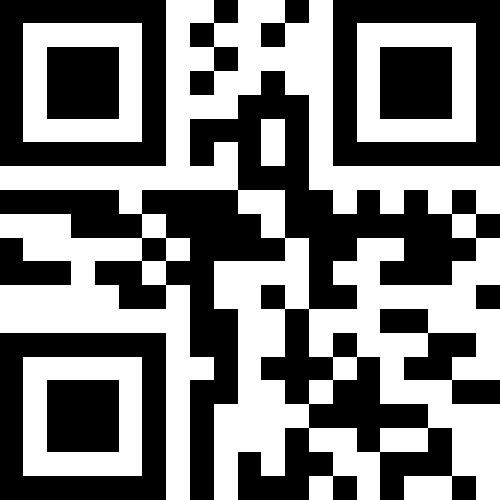
\includegraphics[width=1in]{helloqr.png}
\caption{A QR code with the text ``Hello world!''}
\label{fig:qr:helloqr}
\end{figure}

\begin{table}[t]
\begin{center}
\begin{tabular}{|l|l|l|l|l|l|}
\hline
\pbox[c][25pt][c]{\textwidth}{Error correction \\level} & Data bits & Numeric &	Alphanumeric & Binary & Kanji\\
\hline
L &	23,648 & 7,089 & 4,296 & 2,953 & 1,817\\
\hline
M & 18,672 & 5,596 & 3,391 & 2,331 & 1,435\\
\hline
Q & 13,328 & 3,993 & 2,420 & 1,663 & 1,024\\
\hline
H & 10,208 & 3,057 & 1,852 & 1,273 & 784\\
\hline
\end{tabular}
\caption[Capacities]{Maximum storage capacities for Version-40 codes}
\label{tab:qr:qrcode-capacity}
\end{center}
\end{table}

The capacity of a QR code mainly depends on its data type, version and error correction level. The data type can be \emph{Numeric only},  \emph{Alphanumeric},  \emph{Binary}, or \emph{Kanji}. The version, from 1 to 40, determines a code's dimensions, which range from 21$\times$21 to 177$\times$177 modules. QR codes use a form of error-correction coding which can take four levels: \emph{Low} (L),  \emph{Medium} (M),  \emph{Quartile} (Q), and  \emph{High} (H), as is shown in Table~\ref{tab:qr:qrcode-capacity}. Obviously, as the level increases, more redundancy is introduced in the code's content, which decreases its storage capacity; however, more data can be restored if the code is dirty or damaged. With position detection patterns included in the symbol, a QR code can be decoded in 360 degrees.

Before generating a QR code from a piece of data, a code generator needs to analyze that input data to decide the most efficient mode and version. In the data encoding, the characters are converted into a bit stream, and in this progress, some \emph{mode indicators} and \emph{terminators} are inserted for the mode changes. The bit stream is then split into 8-bit codewords, and pad characters are required to fill the number of codewords for the chosen version. The generated codeword sequence is divided into blocks according to the specific error correction level and an error correction codeword is generated for each block. Then the codewords from each block are interleaved and some remainder bits are added as necessary.

In the next step, the generator places the codeword modules in a black-and-white matrix with the finder pattern, separators, timing pattern and alignment Patterns; it applies the masking patterns, evaluates and then selects the appropriate pattern. Finally, it generates the \emph{Format} and \emph{Version Information} and completes the QR code \citep{iso18004}.

The decoding steps are simply the reverse of the encoding procedure. At first, the QR code needs to be located and the black and white modules are recognized as 0s and 1s that form a binary array. From the binary array, the decoder gets the format information and version information. With that information, it can begin to read the characters and the error correction codewords, and then tries to detect and correct the errors with the error correction codewords according to the appropriate error correction level. In the next step, the data codewords are divided according to the \emph{Mode Indicators} and \emph{Character Count Indicators}, and the data characters are finally decoded and output.

\subsection{The Case for QR code Communication}

The aforementioned process applies for the encoding and decoding of a single code containing static data. We now investigate the idea of using QR codes as a communication channel, where realtime data would be transformed on-the-fly as a \emph{sequence} of QR codes, which could then be optically picked up by some device, and converted back into the original data stream at the receiving end.

The use of QR code communication presents several advantages in a handful of scenarios. For example, the US Navy has investigated the use of QR codes as a ``digital semaphore''. The proposed technology focuses on the detection of low-resolution codes from very long ranges, and highlights the interest and possible use cases for this technology in a military context:

\begin{quote}
Arguably the most significant advantage of QR code LOS [line of sight] communications is the fact that they can be conducted without emitting energy in the RF spectrum. In an emissions controlled (EMCON) environment, this will provide a critical ability to communicate between ships without increasing the possibility of position detection. \citep[p.\ 46]{richter-msc}
\end{quote}

However, in the cited work, the codes are considered to be \emph{static}, i.e.\ they do not change over time to form a stream of data, and more or less act as a substitute for flags or signs. Nevertheless, the absence of any emission of radio waves in QR code communication proves to be an appealing advantage in some scenarios.

We have also seen in the previous section how all other technologies, such as  Bluetooth or IrDA, require dedicated hardware. In contrast, using QR codes to communicate can be done through codes printed on a hard surface, or through any device capable of displaying images in sufficient resolution: TV screens, computer monitors, tablets and cell phones. Similarly, reception can be done through any device equipped with a standard, off-the-shelf camera. This can turn devices equipped with this common hardware into communicating devices, even though they were not designed for that purpose in the first place. One can even imagine emergency situations in which all digital means of communications between two points are not working. If line of sight can be established and a display and a camera are available, the use of QR codes nevertheless makes it possible to transmit digital data ---arguably much faster than the manual handwriting/transcribing that would otherwise need to be done.

\begin{comment}
Preliminary experiments show the technique can work on an inexpensive webcam with a low resolution of $640\times480$ (0.3 megapixels).
\end{comment}

Finally, we have mentioned in the beginning how the use of an optical and strictly one-way communication channel can also be desirable, even in situations where radio or cable communication is available. For example, in the context of runtime verification, the execution of a system is being observed by an external  process called a \emph{monitor}. To prevent the monitor from interfering with the execution of the system, it is often placed on a separate machine, with some communication channel carrying events from the former to the latter. However, in traditional protocols such as TCP, the bidirectional nature of a connection presents too high a risk of attacks on the program to monitor. Moreover, some software setup is required to hook up the monitor to the program: defining IP addresses, pipe names, ports, etc., which represents too much coupling in many scenarios. We have argued in past work \citep{DBLP_conf/rv/LavoieLVGH14} how the use of an optical communication channel can alleviate these problems by providing greater isolation between the system and its monitor.

\subsection{Estimating Bandwidth and Error Rate}

However, one-way transmission introduces the possibility of losing frames during the process, due to the limitation of the physical devices or the vulnerability of the software. Moreover, it is impossible for the transmitter to be aware of any missing frames on the receiving end and resend them. Therefore, we need to analyze thoroughly this approach to estimate the \emph{recognition rate} and the \emph{transmission bandwidth} of such a communication channel.

The transmission of codes takes multiple parameters: each frame's data size, the number of generated frames per second (fps) and the error correction level. All three can have an important effect on the generation of QR codes and the resulting bandwidth. Larger data size leads to a higher symbol version of the QR code and more symbol modules, and with the same frame size, a higher correction level requires more symbol modules than a lower one.

Because the sender cannot be aware of any codes missed by the receiver, this one-way communication channel is actually a lossy channel, of which the \emph{effective} bandwidth can be calculated with the measured frame recognition rate. This represents the number of bits that are correctly received.
%
\begin{equation*}
  bandwidth = \mathit{fps} \times \mathit{frame\_bits} \times \mathit{recognition\_rate}
\end{equation*}

If the receiver finds that not all the frames are received, the only way is to make sure the sender sends all the frames again and again until the receiver gets all frames and stops; the actual bandwidth is:
%
\begin{equation*}
  bandwidth = \mathit{fps} \times \mathit{frame\_bits} \div \mathit{actual\_sent\_times}
\end{equation*}

The recognition rate is normally determined by the ability of the camera and the screen, the accuracy of the recognition algorithm and the code's complexity (i.e.\ the number of the displayed modules). However, within the ability of the camera and the screen, if we can send the same frame for more than once, meanwhile the value of \emph{fps} doesn't need to change, the practical recognition rate can be improved.

\begin{equation*}
\mathit{practical\_recognition\_rate} = 1 - (1 - \mathit{recognition\_rate})^{times}
\end{equation*}


%% }}} --- Section

%% -----------------------
%% Section: expériences
%% -----------------------
\section{Experiments}\label{sec:qr:experiments} %% {{{

In this section, we describe experiments in which we measure the accuracy of reading sequences of QR codes in various conditions. The purpose of these experiments is threefold:

\begin{enumerate}
\item assess whether data can be successfully transmitted through the reading of sequences of optical codes;
\item determine the parameters that maximize the decoding rate and bandwidth of the transmitted data;
\item from these results, determine the characteristics of a typical QR stream communication channel.
\end{enumerate}

\subsection{Experimental Setup}

Our set of experiments involves producing and displaying sequences of QR codes on one end, and capturing and decoding these sequences on the other. In our experimental environment, we used a Samsung 19-inch LED monitor as the transmitter and a high-definition Logitech webcam as the receiver. The camera was placed at a fixed distance of 50 cm from the screen. The resolution of the monitor was 1280$\times$1024 pixels. %The webcam can capture at most 30 frames per second with the highest resolution of 1920 pixels $\times$ 1080 pixels. Zooming was disabled. 
The camera was placed on a stable surface, with the optical code zone correctly in focus and covering the whole field of view. The computer used for the experiments is a laptop with the Intel Core i7-3632QM processor and 16 GB of memory. Figure \ref{fig:qr:setup} shows the setup used for the experiments.

\begin{figure}
\centering
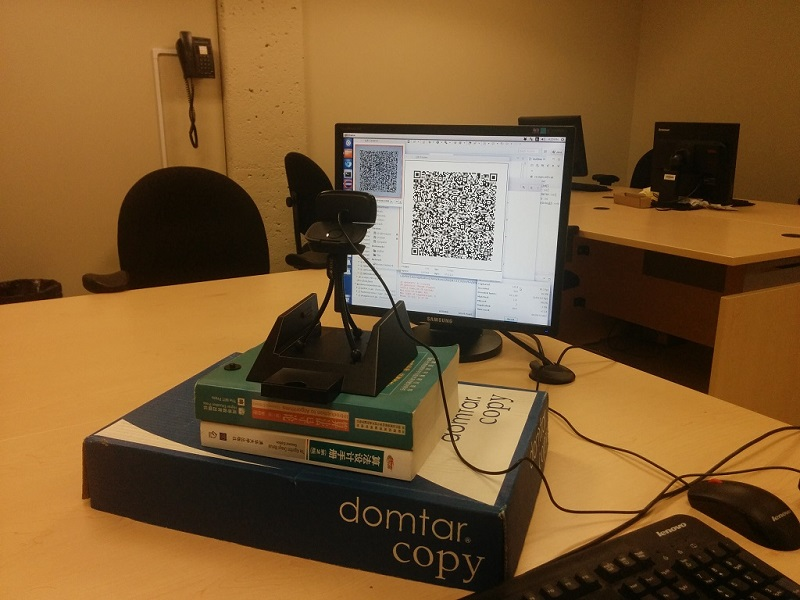
\includegraphics[width=\linewidth]{expsetup.jpg}
\caption{Experimental setup for reading codes.}
\label{fig:qr:setup}
\end{figure}

In the development, we chose OpenCV\footnote{\url{http://opencv.org/}} to capture the images from the camera and ZXing\footnote{\url{https://github.com/zxing/zxing}} to generate and decode the QR codes. To reduce the CPU and memory's overhead of capturing and decoding, the captured images were transformed to 16-level grayscale. The data used to generate QR codes were randomly generated \emph{alphanumerics}. All benchmarking code is implemented in Java and is freely available.\footnote{\url{http://github.com/sylvainhalle/GyroGearloose}}

The code decoding depends on the quality and the complexity of the captured image. If the image is broken or blurred, it will be difficult to decode. And the algorithms of image recognition may have the probability of failure\citep{adel2006}. Therefore, our first step is to measure the ability of optical recognition libraries to properly read sequences of codes, irrespective of the actual data contained in these codes. Sequences of codes were generated by producing a character string of the form \verb+dddd#rrrr...+, where \verb+dddd+ is a sequential number starting from zero and incrementing by one on each successive code, and \verb+rrrr...+ is a random string of characters (different on each code) long enough to fill the code up to its maximum size. Each test consisted in filming the sequence of such codes and storing the sequential number of each correctly decoded image into a file. This allows us to determine the fraction of all codes that were correctly read; given the size of each code and the number of codes sent, this makes it possible to compute the bandwidth and decoding error rate.

Our experiments quickly tripped over what appears to be a bug in the ZXing image decoding library. When analyzing sequences of images captured by the camera to look for decoding errors, we discovered that a number of times, the decoding failed while the corresponding image seemed to have no apparent problem (no blurring, correct framing, etc.). Putting the offending codes back on screen and trying to properly decode them with the camera yielded no success, even after changing the code's size, the camera's position, lighting conditions, etc. This is all the more puzzling that codes immediately before and after the problematic one were correctly decoded in multiple frames, while being captured in the same conditions. Even sending the code's ``pure'' image directly back into the decoding algorithm, without going through a camera, produces a decoding error.

It therefore seems the library cannot recognize some of the codes it itself produces (Figure \ref{fig:qr:bad-code} shows such an example). This most probably indicates a bug in the library, which has persisted up to the latest version available at the time this chapter was written. Therefore, in the following, the reader should keep in mind that an unknown proportion of reading errors may be due to this purported bug, and not to the particular experimental conditions. This is the case, for example, for the gaps in the correction rate we shall observe in Figures \ref{img-exp1} and \ref{img-exp2}.

\begin{figure}
\centering
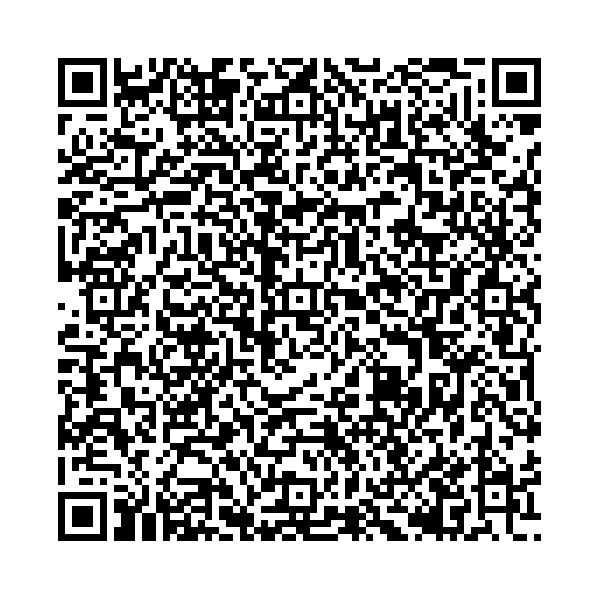
\includegraphics[width=.8\linewidth]{badqr.png}
\caption{A QR code generated by ZXing that ZXing itself cannot decode in the experiment.}
\label{fig:qr:bad-code}
\end{figure}

\subsection{Experimental Parameters}

The experiment seeks the combination of parameters that could maximize the bandwidth and minimize the error rate for the transmission of codes. The parameters that were considered are the following.

\subsubsection{Code Resolution}

The first parameter is code data size (i.e.\ the number of data bits contained in each code) and physical size (number of pixels used to display the code on screen). We varied the data size in increments of 500 bits, from 500 up to 4,500 bits. As shown in Table \ref{tab:qr:sample-sizes}, the largest QR code, which contains 4,500 bits of data using the highest error correction level, is 101$\times$101 modules large. We also fixed the code's physical size to 700$\times$700 pixels, which makes each module a square of at least 6$\times$6 pixels.

\begin{table}[ht]
\begin{center}
\begin{tabular}{llll}
Input data bits & Error correction level & Symbol version & Symbol size\\
\hline
\multirow{2}{*}{500} & L & 3 & 29$\times$29\\
& H & 5 & 37$\times$37\\
\hline
\multirow{2}{*}{1000} & L & 5 & 37$\times$37\\
& H & 9 & 53$\times$53\\
\hline
\multirow{2}{*}{1500} & L & 6 & 41$\times$41\\
& H & 11 & 61$\times$61\\
\hline
\multirow{2}{*}{2000} & L & 8 & 49$\times$49\\
& H & 13 & 69$\times$69\\
\hline
\multirow{2}{*}{2500} & L & 9 & 53$\times$53\\
& H & 15 & 77$\times$77\\
\hline
\multirow{2}{*}{3000} & L & 10 & 57$\times$57\\
& H & 17 & 85$\times$85\\
\hline
\multirow{2}{*}{3500} & L & 11 & 61$\times$61\\
& H & 18 & 89$\times$89\\
\hline
\multirow{2}{*}{4000} & L & 12 & 65$\times$65\\
& H & 20 & 97$\times$97\\
\hline
\multirow{2}{*}{4500} & L & 13 & 69$\times$69\\
& H & 21 & 101$\times$101\\
\hline
\multirow{2}{*}{5800} & L & 19 & 93$\times$93\\
& H & 30 & 137$\times$137\\
\hline\end{tabular}
\caption[Sample sizes]{Sample QR code sizes, according to their data size and error correction level \citep{iso18004}}
\label{tab:qr:sample-sizes}
\end{center}
\end{table}

\subsubsection{Code Rate}

The second experimental parameter we considered is the code rate, i.e.\ the number of codes displayed per unit of time. We initially selected 2, 4, 6, 8, and 10 codes per second (cps), and also considered up to 16 cps in a later phase of the experiment.

\subsubsection{Error Correction Level}

As we have seen, QR codes include additional data intended for error correction. We hence also varied the level of error correction used in each experiment, using either its highest setting (H) or its lowest (L).

\subsubsection{Camera Resolution and Rate}

The resolution of the camera was not considered as an experimental parameter. It was fixed to its maximal setting, 1920$\times$1080 pixels. Similarly, its frame rate was kept fixed at 30 frames per second. This corresponds to 1080p high-definition video, a setting expected to be found in the majority of recent and future video capture devices. We performed some informal tests with lower resolutions (down to 640$\times$480), which were globally conclusive, but did not deem relevant of including them in our detailed analysis.

\subsection{Experimental Results}

The product of all combinations of code size, error correction level and code rate produces a total of 90 different experiments. These experiments were repeated in three sets, differing in the way in which codes were displayed.

\subsubsection{Single Display}

In a first experiment, each code was displayed in sequence for a duration of $1/f$ second, where $f$ is the code rate. The bandwidth and decoding rate are shown in Figure \ref{img-exp1} for combinations of all parameters.

\begin{figure}
\begin{center}
\centering
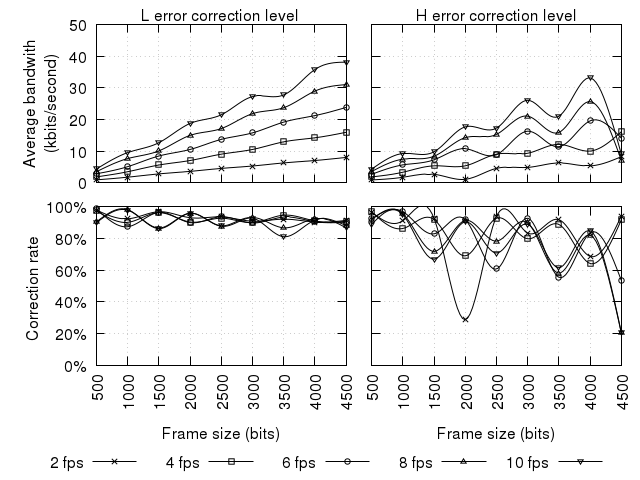
\includegraphics[width=\linewidth]{data1.png}
\caption{Bandwidth and decoding rate in the first experiment}
\label{img-exp1}
\end{center}
\end{figure}

As one can see, the recognition rates of higher correction level were lower than the ones of lower correction level, with all other parameters being equal. This can be explained by the fact that the same amount of data, carried inside a code with a higher correction level, has to display more modules. For example, according to Table \ref{tab:qr:sample-sizes}, the modules of a 2,000-bit, H-level code are as small as those of a 4,500-bit, L-level code. Smaller modules, in turn, yields increased difficulty in recognition by the camera. Therefore, a first conclusion one can draw is that, surprisingly, effective bandwidth seems to be improved by using a \emph{lower} level of error correction.

With the same data sizes and correction levels, the figure shows that the recognition rate decreases as the code rate increases. This can be explained by the fact that, in a higher code rate, the same code occupies fewer camera frames, and hence has fewer chances of being correctly decoded in one of the frames. Moreover, the probability that a code change occurs at the moment a frame is taken (resulting in a blurry image showing part of two different codes) is also increased. In the L level, the decrease is slight, but in the H level, the decrease is dramatic when the code size reaches 3,000 bits. As the data size increases, the recognition rate drops constantly and considerably.

These figures seem to indicate that the ideal configuration for level L is 4,500 bits and 10 fps, which yields an effective bandwidth of 39.0 kbps; for level H, 4,000 bits and 10 fps result in a bandwidth of 24.6 kbps.

\subsubsection{Double Display}

Considering that the camera might have missed several frames, we performed a second experiment in which every QR code is displayed twice within a small time window. Hence, instead of displaying each code once for $1/f$ second, each code was interleaved with neighbouring codes and displayed twice for $1/2f$ second each time. This results in the same total exposure time for each code, but increases the diversity in the images captured by the camera.

\begin{figure}[ht]
\begin{center}
\centering
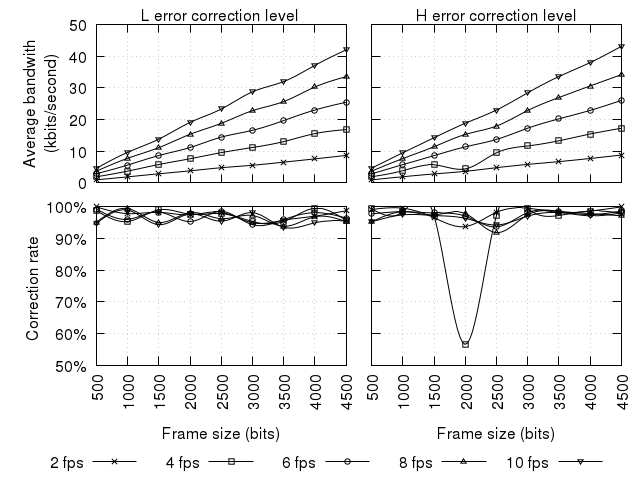
\includegraphics[width=\linewidth]{data2.png}
\caption{Bandwidth and decoding rate in the second experiment, where each code is displayed twice}
\label{img-exp2}
\end{center}
\end{figure}

The results are plotted in Figure \ref{img-exp2}. They show an increase in all recognition rates, which are now all higher than 90\%. This, in turn, increases the effective bandwidth; using the same settings as above, one can get a bandwidth of 43.0 kbps using level L, and 44.1 kbps using level H.

\subsubsection{Random Padding}

However, as we discussed earlier, not all QR codes are created equal; for the same resolution and error correction level, experimental results indicate that some codes seem to be more difficult to read than some others. Therefore, merely repeating the same image multiple times has no impact on that intrinsic ``hardness''. Our third experiment introduces yet another mechanism for boosting recognition rate.

This time, we tried to make the codes from the same input data different by appending, at the end of the data to be encoded, a small random string intended to change every time the code is to be displayed. Hence the same original data, if displayed twice, is prepended to a different random padding each time, yielding a slightly different array of bits. However, by virtue of the QR encoding schema, even a small change at the end of an array produces a completely different pattern of dots in the resulting QR code. Figure \ref{fig:qr:difcodes} shows an example of this phenomenon. Therefore, if a code is harder to read, the same data is also displayed in a largely different pattern of dots, increasing the odds of being properly picked up at least once.

\begin{figure}
\centering
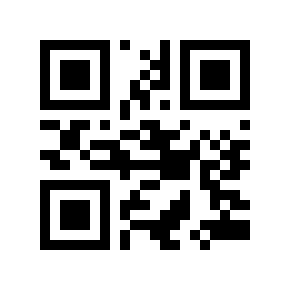
\includegraphics[width=1in]{abcdefg.jpg}~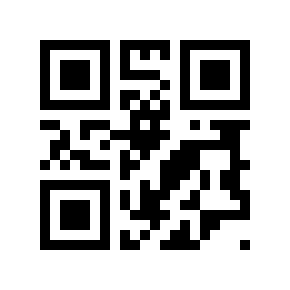
\includegraphics[width=1in]{abcdeff.jpg}
\caption{Examples of two codes with slightly different data, but widely different dot patterns. The code on the left contains the string ``abcdefg'', while the one on the right contains ``abcdeff''.}
\label{fig:qr:difcodes}
\end{figure}

Although the objective reason for some codes being harder to read is unknown and out of the focus of this chapter, experimental results seem to confirm this hypothesis. We performed a third experiment where every input data was displayed three times with different generated QR codes. The recognition rate is better than before when the code rate is lower than 10 fps, as shown in Figure \ref{img-exp3}. % the best bandwidth in L level is 44.9 kbps and in H level is 43.4 kbps.

\begin{figure}[ht]
\begin{center}
\centering
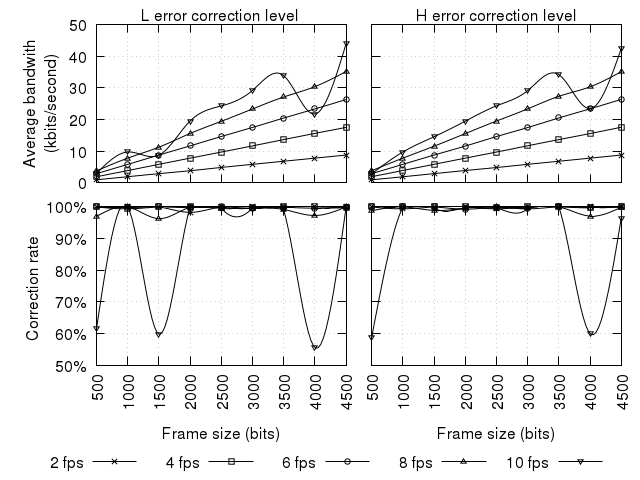
\includegraphics[width=\linewidth]{data3.png}
\caption{Third experiment: triple display and random padding}
\label{img-exp3}
\end{center}
\end{figure}

These results led us to experiment with higher code rates; we added 12 cps, 14 cps and 16 cps. The codes were displayed twice. As the Figure \ref{img-exp4} shows, the maximum effective bandwidth in the result is 65.5 kbps using level L, and 68.3 kbps in level H level, using 16 cps and 4,500-bit codes.

\begin{figure}[ht]
\begin{center}
\centering
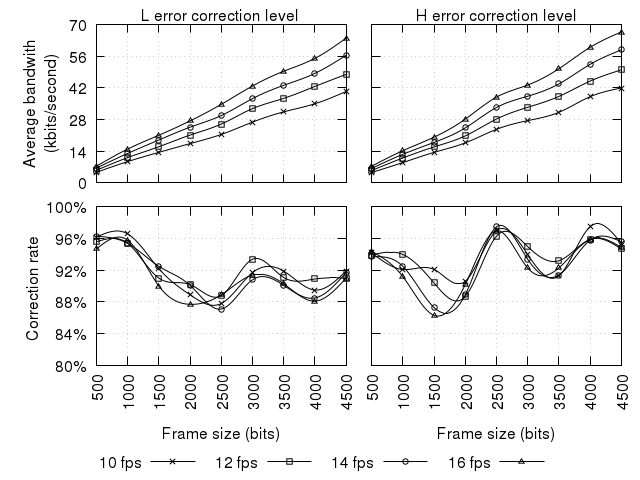
\includegraphics[width=\linewidth]{data4.png}
\caption{Fourth experiment: double display and higher code rates}
\label{img-exp4}
\end{center}
\end{figure}

\subsection{Partial Conclusions}

These initial experiments allow us to draw a few conclusions on the nature of a QR-based communication channel. First, although higher code rate and code size have a negative impact on the recognition ratio, the increased data that can be carried globally compensates for the higher error rate in terms of \emph{effective} bandwidth. Second, introducing repetition and varying the dot pattern for the same data increases the effective bandwidth; that is, showing two different codes for half the time is more effective than a single code for the same interval. Third, even for the smallest code sizes, the error rate of the channel is never zero, indicating that the channel is intrinsically lossy. 

From these findings, one can reasonably expect a QR code stream to provide a channel with an effective bandwidth of about 40 kbps, when displaying 10 4,000-bit codes per second using the random padding technique and L-level error correction. The decoding rate of the channel using these parameters should be of at least 95\%. Obviously, these findings apply to a fixed-camera setting. They do not take into account potential jitter, blurring or other effects that may occur in other contexts ---although an informal experiment described in Section \ref{subsub:swipe} tends to indicate the technology is relatively robust.

%% }}} --- Section

%% -----------------------
%% Section: le protocole
%% -----------------------
\section{A Protocol for One-Way, Lossy Communication Channels}\label{sec:qr:protocol} %% {{{

In this section, we propose an approach which uses continuous QR codes as a medium to achieve one-way data transmission.

\subsection{Design Goals}

In order to implement a communication channel, a specific protocol is essential; it should be well designed so that the data can be serialized and transferred without significant overhead. Besides, the protocol has to have the ability of splitting the to-be-transferred data into frames to generate the QR images. The result is BufferTannen, a Java software package dedicated to the serialization and transmission of structured data over limited communication channels.\footnote{\url{https://github.com/sylvainhalle/BufferTannen}} It provides a set of classes allowing the representation of structured data in a compact binary form. Contrarily to other systems, like Google's Protocol Buffers \footnote{\url{https://github.com/google/protobuf}}, defining new message types can be done at runtime and does not require compiling new classes to be used. Moreover, messages in BufferTannen cannot be encoded and decoded without prior knowledge of their structure. However, since messages do not contain information about their structure, they use much less space.

BufferTannen also defines a protocol allowing the transmission of messages.  Although any channel (TCP connection, etc.) can be used, BufferTannen was designed to operate on a channel with the following specifications, which are based on our initial experimental results:

\begin{itemize}
\item The channel is \emph{point-to-point}. The goal is to send information   directly from A to B; no addressing, routing, etc. is provided.
\item The channel is \emph{low-bandwidth} (that is, able to transmit a few hundred bytes at a time, possibly less than 10 times per second).
\item The channel is \emph{one-way}: typically, one side of the communication sends data that is to be picked up by some receiver. This entails that the receiver cannot acknowledge reception of data or ask the sender to transmit again, as in protocols like TCP.
\item The channel is \emph{lossy}. However, we assume that the channel provides a mechanism (such as some form of checksum) to detect when a piece of data is corrupted and discard it.
\item A receiver can start listening on the channel at any time, and be able to correctly receive messages from that point on. As such, the communication does not have a formal ``start'' that could be used, for example, to advertise parameters used for the exchange.
\end{itemize}

Therefore, the communication channel envisioned as the transmission medium for BufferTannen's messages can be likened in many ways to a slow broadcast signal, such as Hellschreiber \citep{hells}, slow-scan television \citep{slowtv}, Teletext \citep{teletext} or RBDS~\citep{rbds}.

BufferTannen's protocol aims at transmitting messages as reliably as possible under these conditions, while preserving the integrity of data and the ordering of messages. The low-bandwidth nature of the channel explains the emphasis on serializing messages in a compact binary form. Since the receiver cannot ask for any form of re-transmission, the protocol must provide for automatic re-transmissions of each message to maximize their chances of being picked up, while at the same time not confusing a re-transmission with a new message with identical content. Moreover, as the receiver can start listening at any moment, and that the schema of messages must be known in order to decode them, the schemas used in the communication must also be transmitted at periodic intervals.

\subsection{Schemas}
\setcounter{paragraph}{0}

The declaration of a data structure is called a \emph{schema}. Information can be represented in three different forms:

\begin{itemize}
\item Smallscii: A variable-length string of characters. Since BufferTannen is aimed towards limiting as much as possible the number of bits required to represent information, these strings are restricted to a subset of 63 ASCII characters (letters, digits and punctuation). Each character in a Smallscii string takes 6 bits, and each string ends with the 6-bit string \verb+000000+.

\item Integer: The only numerical type available in BufferTannen. When declared, integers are given a ``width'', i.e. the number of bits used to encode them. The width can be anything between 1 and 16 bits.

\item Enumeration: A list of predefined Smallscii constants. Enumerations can be used to further reduce the amount of space taken by a data element when its set of possible values is known in advance.
\end{itemize}

These basic building blocks can be used to write schemas by combining them using compound data structures:

\begin{itemize}
\item List: a variable-length sequence of elements, all of which must be of the same type (or schema). List elements are accessed by their index, starting
  with index 0.
\item FixedMap: a table that associates strings to values. The structure is fixed and the exact strings that can be used as keys must be declared. However, each key can be associated to a value of a different type.
\end{itemize}

These constructs can be mixed freely. The following represents the declaration of a complex message schema:

\begin{verbatim}
FixedMap {
  "title" : Smallscii,
  "price" : Integer(5),
  "chapters" : List [
     FixedMap {
       "name" : Smallscii,
       "length" : Integer(8),
       "type" : Enum {"normal", "appendix"}
     }
  ]
}
\end{verbatim}

The top-level structure for this message is a map (delimited by \verb+{+\dots\verb+}+). This map has three keys: \verb+title+, whose associated value is a Smallscii string, \verb+price+, whose associated value is a integer in the range 0-32 (i.e. 5 bits), and \verb+chapters+, whose value is not a primitive type, but is itself a list (delimited by \verb+[+...\verb+]+). Each element of this list is itself a map with three keys: a string \verb+name+, an integer \verb+length+, and \verb+type+ whose possible values are \verb+normal+ or \verb+appendix+.

Schemas can be represented in a compact and unequivocal binary representation as follows.

\paragraph{Integer} The declaration of an integer is encoded as the following sequence of bits:
%
\begin{verbatim}
ttt wwwww ddddd s
\end{verbatim}

The sequence \verb+ttt+ represents the element type, encoded on 3 bits. An integer contains the decimal value 6. The sequence of \verb+w+ indicates the integer's width in bits. The width itself is encoded over 5 bits. The sequence of \verb+d+ indicates the integer's width, in bits, when expressed as a delta value, i.e.\ as the difference with respect to an integer from a previous message. The width itself is encoded over 5 bits. The single bit \verb+s+ is the sign flag. If set to 0, the integer is unsigned; if set to 1, the integer is signed. Note that integers expressed as delta values are always encoded as signed integers; hence this flag only applies to integers occurring as full values.

\paragraph{Smallscii string} The declaration of a Smallscii string is simply coded as three bits representing the element type; a string contains the decimal value 2.

\paragraph{Enumeration} An enumeration must provide the list of all possible values it can take. It is formally represented as:
%
\begin{verbatim}
ttt llll [ssssss ssssss ... 000000 ...
 ssssss ssssss ... 000000]
\end{verbatim}

The element type is the decimal value 1, and the sequence \verb+llll+ is the number of elements in the enumeration, encoded on 4 bits. What follows is a concatenation of Smallscii strings defining the possible values for the enumeration. Each character is encoded on 6 bits, and the end of a string is signalled by the 6-bit sequence \verb+000000+.

\paragraph{List} The declaration of a list is as follows:
%
\begin{verbatim}
ttt llllllll ...
\end{verbatim}

The element type is the decimal value 3; the 8-bit sequence \verb+llllllll+ defines the maximum number of elements in the list. What follows is the declaration of the element type for elements of that list.

\paragraph{Fixed Map} The last element type is the fixed map, declared as follows:
%
\begin{verbatim}
ttt [ssssss ssssss ... 000000 ddd...]
\end{verbatim}

The element type is the decimal value 4; what follows is a Smallscii string defining the name of a key, followed by the declaration of the element type for that key; this is repeated for as many keys the map declares.

\subsection{Messages}
\setcounter{paragraph}{0}

A \emph{message} is an instance of a schema. For example, the following is a possible message abiding by the previous schema:

\begin{verbatim}
{
  "title" : "hello world",
  "price" : 21,
  "chapters" : [
    {
      "name" : "chapter 1",
      "length" : 3,
      "type" : "normal"
    },
    {
      "name" : "chapter 2",
      "length" : 7,
      "type" : "normal"
    },
    {
      "name" : "conclusion",
      "length" : 2,
      "type" : "appendix"
    }
  ]
}
\end{verbatim}

The reader familiar with JSON or similar notations will notice strong similarities between BufferTannen and these languages. As a matter of fact, elements of a message can be queried using a syntax similar to JavaScript. For example, assuming that \verb+m+ is an object representing the above message, fetching the length of the second chapter would be written as the expression:

\begin{verbatim}
m[chapters][1][length]
\end{verbatim}

This fetches the \verb+chapters+ value in the top-level structure (a list), then the second element of that list (index 1), and then the \verb+length+ value of the corresponding map element.

As with schemas, messages can be represented in a compact binary form.

\paragraph{Smallscii string} Strings are represented as a sequence of 6-bit characters, terminated by the end of string delimiter \verb+000000+.

\paragraph{Integer} Numbers are represented by the sequence of bits that encodes their value, without any terminating sequence: the number of bits to read is dictated by the size of the integer, as specified by the corresponding schema element. If the integer is signed, the first bit represents the sign (0 = positive, 1 = negative) and the remainder of the sequence represents the absolute value. %(Yes, this means that there are two ways of encoding 0 in a signed integer, either as -0 or as +0. Both will correctly be decoded as 0.)

\paragraph{Enumeration} An enumeration is simply made of the sequence bits corresponding to the appropriate value. Again, the number of bits to read is dictated by the size of the enumeration, as specified in the schema of the message to read. For example, if the enumeration defines 4 values, then 2 bits will be read. The numerical value $i$ corresponds to the $i$-th string declared in the enumeration.

\paragraph{List} A list begins by 8 bits recording the number of elements in the list. The remainder of the list is the concatenation of the binary representation of each list element. Since the type of each element and the number of such elements to read are both known, no delimiter is required between each element or at the end of the list.

\paragraph{Fixed Map} The contents of a fixed map is simply the concatenation of the binary representation of each map value. The key to which each value is associated, and the value type to read, are specified in the schema of the message to read, and are expected to appear exactly in the order they were declared. This spares us from repeating the map's keys in each message.

\subsection{Reading and Writing Messages}

In BufferTannen, both schemas and instances of schemas are represented by the same object, called \verb+SchemaElement+. An empty SchemaElement must first be instantiated using some schema; this can be done by either:

\begin{itemize}
\item Reading a character string formatted as above; or

\item Reading a binary string containing an encoding of the schema. As a matter of fact, in BufferTannen both messages \emph{and} schemas can be transmitted in binary form over a communication channel, and a method is provided to export the schema of some message into a sequence of bits.
\end{itemize}

Once an empty SchemaElement is obtained, it can be filled with data, again in two ways:

\begin{itemize}
\item By reading a character string formatted as above; or

\item By reading a binary string containing an encoding of the data.
\end{itemize}

Similar methods exist to operate in the opposite way, and to \emph{write} a message's schema or data contents either as a character string or as a binary string. This way, messages and schemas can be freely encoded/decoded using human-readable text strings or compact binary strings.

As one can see, for a message to be read or written, it is necessary first to instantiate an object with a schema. As a matter of fact, trying to decode a stream of data without first advertising the underlying schema will cause an error, even if the stream contains properly formatted data. Similarly, trying to read data that uses some schema with an object instantiated with another schema will also cause an error. In other words, no data can be read or written without knowledge of the proper schema to use.

This might seem restrictive, but it allows BufferTannen to heavily optimize the binary representation of messages. In the absence of a known schema, each message would require to carry, in addition to its actual data, information about its own structure. %Since a reader receiving a sequence of bits would not know in advance how to read it, special sequences would need to be added to notify the reader that what follows is a map with some number of keys, and then in turn each value for each key would also need to declare the structure of its own type, and so on.
%
Practically speaking, this amounts to repeating within each message the description of its schema, interspersed through the message data. On the contrary, if the schema is known, all this signaling information can be discarded: when receiving a sequence of bits, a reader that possesses the schema knows exactly how many bits to read, what data this represents and where to place it in the message structure being populated. This entails, however, that a receiver that does not know the schema to apply has no clue whatsoever on how to process a binary string.

To illustrate the interest of BufferTannen as a message encoding scheme, we consider the example of transmitting events from a video game to an external monitor.

\subsection{Segments}
\setcounter{paragraph}{0}

Messages and schemas are encapsulated into a structure called a \emph{segment}. A segment can be of four types:

\paragraph{Message segments} contain the binary representation of a message, along with a sequential number (used to preserve the ordering of messages received), as well as the number referring to the schema that must be used to decode the message. A message segment consists of a header structured as follows:

\begin{verbatim}
tt nnnnnnnnnnnn wwwwwwwwwwww ssss ...
\end{verbatim}

The header starts with two bits describing the type of the segment; a message segment contains the decimal value 1. The \verb+n+ and \verb+w+ sections describe the segment's sequential number and total length, both encoded on 12 bits. The four \verb+s+ bits provide the schema number in the schema bank that should be used to read this segment. The remainder of the segment is comprised of a map, list, Smallscii string or number, whose binary representation was described above.

\paragraph{Schema segments} contain the binary representation of a schema, which is associated to a number. Multiple schemas can be used in the same communication, hence creating a bank of schemas identified by their number. A schema segment consists of a header structured as follows:

\begin{verbatim}
tt nnnnnnnnnnnn ssss ...
\end{verbatim}

The header starts with two bits describing the type of the segment; a schema segment contains the decimal value 2. The \verb+n+ section describes the segment's sequential number, and the \verb+s+ section gives the the schema number in the schema bank this segment should be assigned to. The remainder of the segment is comprised of a binary string describing the schema, whose representation was described above.

\paragraph{Blob segments} are intended to carry raw binary data over the BufferTannen protocol.

\paragraph{Delta segments} contain the binary representation of a message, expressed as the difference (``delta'') between that message and a previous one used as a reference. Delta segments are used to further compress the representation of a message, in the case where messages don't change much over an interval of time.

\begin{verbatim}
tt nnnnnnnnnnnn wwwwwwwwwwww rrrrrrrrrrrr...
\end{verbatim}

The header starts with two bits describing the type of the segment; a delta segment contains the decimal value 1. The \verb+n+ and \verb+w+ sections describe the segment's sequential number and total length, both encoded on 12 bits. The \verb+r+ section gives the sequential number of another segment, relative to which the delta of the current segment are expressed. What follows is a binary string that describes the ``difference'' one must compute with respect to that segment to obtain the contents of the current one.

The computation of the delta is performed recursively on each element of the two messages to compare in the order they occur. It is defined for each element type as follows.

\begin{itemize}
\item Smallscii strings: if the corresponding strings are identical, emit the single bit \verb+0+. Otherwise, emit the bit \verb+1+ followed by the Smallscii string of the target message.
%
\item Integers: if the corresponding numbers are identical, emit the single bit \verb+0+. Otherwise, emit the bit \verb+1+ followed by the difference between the source and the target integer.
%
\item Enumerations: if the corresponding value of the enumerated type is the same, emit the single bit \verb+0+. Otherwise, emit the bit \verb+1+ followed by the integer value corresponding to the index of the value in the target message.
%
\item Lists: if both lists have the same elements in the same order, emit the single bit \verb+0+. Otherwise, emit the bit \verb+1+ followed by the binary representation of the target list.
%
\item Maps: recursively apply the previous rules for each key of the map.
\end{itemize}

One can see that delta segments apply only a coarse form of comparison. For example, no attempt is made to detect whether two lists differ by the addition or deletion of an element; the contents of the list is retransmitted in full whenever it is not identical to the original. Nevertheless, this technique allows substantial savings whenever a part of a data structure remains identical from one message to the next.

\subsection{Frames}
\setcounter{paragraph}{0}

The communication channel sends binary data in units called \emph{frames}. A frame is simply a set of concatenated segments in binary form, preceded by a header containing the version number of the protocol (currently ``1'') and the length (in bits) of the frame's content. Formally, the binary structure of a frame is as follows:

\begin{verbatim}
vvvv nnnnnnnnnnnnnn ffff... ffff...
\end{verbatim}

The \verb+v+ section consists of the 4-bit protocol version number, followed by 14 bits indicating the total length (in bits) of the frame. Each segment is appended directly to this 18-bit header. As each segment's header contains its own length, no further marshaling is required to correctly decode segment data.

When many segments are awaiting to be transmitted, the protocol tries to fit as many segments as possible (in sequential order) within the maximum size of a frame before sending it. This maximum size can be modified to fit the specifics of the communication channel that is being used. In the current incarnation of the protocol, segments cannot be fragmented across multiple frames. Hence a segment cannot exceed the maximum size of a frame.

Each frame is then converted into a QR code, with its binary content Base64-encoded as the code's text. This QR code can then be read at the receiving site, converted into a binary sequence, and parsed back into frames, segments and messages by applying the reverse transformations.

\subsection{Streaming Modes}
\setcounter{paragraph}{0}

BufferTannen is designed with two sending modes, respectively called ``Lake'' mode and ``Stream'' mode.

Lake mode is intended for the sending of a finite piece of data, such as a file, or a sequence of BufferTannen messages whose complete contents are known in advance. The data to be sent is divided into a finite set of segments, and the whole sequence of segments is repeatedly emitted through QR codes. If any frames are missed or incorrectly decoded, the infinite repetition of all segments makes possible to catch the missing data at the next loop. Ultimately, decoding errors may entail that the data needs to be read for more than one loop before it is completely received.

The use of Lake mode can be detected by frames carrying a non-zero value to their ``total segments'' header field. Hence a receiver that starts reading at any point through the sequence of frames knows how many segments in total are to be received, and the relative position of each segment in the data to be reconstructed. This makes Lake mode a relatively slow, but very robust optical data transmission scheme.

In Stream mode, the data is continuously read into segments which then form a stream of frames, and the frames are immediately sent. The reading process stops only when there is no more data to read. The frames already sent are removed from the memory, so there is no way to resend the data for several times. However, for the sake of the data consistency, we made a buffer for the clones of the sent frames, and after having sent a specific amount frames fetched from the original data, the frames in the buffer are resent again and then removed from the buffer. Therefore, Stream mode is intended to send realtime data, typically where where the data loss is acceptable and the consistency can be slightly sacrificed (e.g.\ audio or video).

\begin{figure*}
\centering
\begin{verbatim}
--------------------------------------------------------------------------
Sending mode:        lake
Buffer state:        [||>       ||:.::||:|||] 59% (130/219)
Progress:            0408/0000 (13.8 sec @30 fps)
Link quality:        22/30 [*******   ] (73%)  Global:   339/454 (74%)
Data stream index:   0
Resource ident.:     myfile.jpg
Processing rate:     35 ms/frame (27 fps)
--------------------------------------------------------------------------
\end{verbatim}
\caption{Part of the text interface of the QR code receiver operating in Lake mode}
\label{fig:qr:lake-gui}
\end{figure*}

Figure \ref{fig:qr:lake-gui} shows a portion of the text interface of our QR code receiver implementation. The interface shows that the frames being received are in Lake mode. The buffer state field indicates the progress of the reception. In the example, it shows that 130 out of 219 segments have been correctly received; the text bar at the left indicates to what portions of the total sequence these segments correspond. A section of the sequence that has not been received at all is indicated by a blank space; increasingly full portions of the sequence are represented respectively by the symbols \verb+.+, \verb+.+ and \verb+|+. The \verb+>+ symbol indicates the relative position of the last segment that was correctly read.

The ``Link quality'' field gives a realtime indication of the decoding rate. It shows that 22 of the last 30 images captured by the camera were correctly decoded, and that globally, 339 images were decoded out of 454 captured. The resource identifier and data stream index, carried by each frame, is also displayed.

\subsection{Experimental Results}
\setcounter{paragraph}{0}

The experiments of Section \ref{sec:qr:experiments} confirmed our intuition that optical code streams are an inherently unreliable and low-bandwidth communication channel. The compactness of the BufferTannen protocol can be motivated by an example from runtime verification. A particular video game, called Pingus, was instrumented to produce events containing the state of every character in the game. The schema for these events is shown in Figure \ref{fig:qr:pingus-schema}.

\subsubsection{File Transfer}

\begin{figure}
\centering
\begin{verbatim}
FixedMap {
  "pingus" : List [
    FixedMap [
      "id" : Integer(6),
      "x" : Integer(10),
      "y" : Integer(10),
      "velocity-x" : Integer(4),
      "velocity-y" : Integer(4),
      "state" : Enum {"floater",
         "basher", "builder",
         "athlete", "normal"}
    ]
  ]
}
\end{verbatim}
\caption{The schema of events produced by an instrumented video game.}
\label{fig:qr:pingus-schema}
\end{figure}

An event typically contains data for 50 characters, hence the map structure is repeated that many times. Sending such an event in clear-text format, without any whitespace, takes roughly 3,750 bytes. At a rate of 30 events per second, it takes 879 kbps of bandwidth to transmit the event stream. The same event in BufferTannen takes 1,856 \emph{bits}, or 232 bytes. This divides by more than 16 the bandwidth requirements for sending a stream of such events, yielding a bandwidth of 54 kbps.\footnote{Sending the same character string into Gzip shrinks it down to 716 bytes, which makes standard compression a less appealing alternative in that context.} From that point on, delta segments can be used to further reduce the stream's bandwidth, and transmit the remaining events using slightly more than 100 bytes each, consuming a bandwidth of approximately 24 kbps. Our previous experiments show that this is within the range of what one can reasonably expect to transmit using QR codes.

We then tested the ability of the BufferTannen protocol to mitigate these defects, through its use of repetition and its compact binary representation.\footnote{A video of BufferTannen in action is available online: \url{https://www.youtube.com/watch?v=GSL0md0TlY8}}

We chose to encode data into 4,000-bit codes, which, after the encapsulation of BufferTannen, amounts to a QR code of about 5,800 bits. With the combination of 5800 bits and L correction level, according to Table \ref{tab:qr:sample-sizes}, the symbol size is about 93 $\times$ 93 which is between the combinations of 3,500-bit, H-level and 4,000-bit, H-level. From the result of the last experiment, the combinations of 4,000-bit, H level and any sample fps has more than 95\% correction rate which is reliable. Secondly, the code rates were 4, 6, 8, 10, 12 fps. According to the last experiment, this configuration is reliable and supposed to be able to supply 23.2--69.6 kbps, and 16.0--48.0 kbps of bandwidth, respectively.
%
In the consideration of the practical application, we chose to transfer a sample file of which the size is 37,656 bytes, and we performed each experiment 20 times.

The result of the Lake mode experiment in Figure \ref{img-explake} shows that the best fps value is 10, and in this case the sample file needed to be transferred on average 2.4 times to make sure that the receiver could get all the frames. The average spent time is 17.27 seconds, from which the bandwidth is about 17.0 kbps.

\begin{figure}[ht]
\begin{center}
\centering
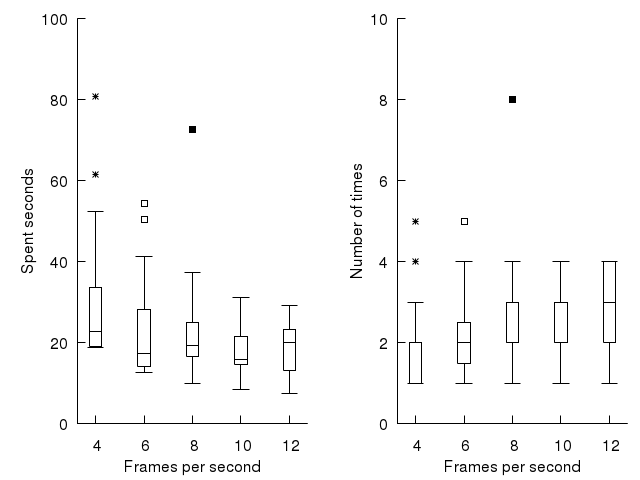
\includegraphics[width=\linewidth]{lake.png}
\caption{Time to send data in Lake mode}
\label{img-explake}
\end{center}
\end{figure}

In Stream mode, the percentage of received codes is important. In the experiment, according to Figure \ref{img-expstream}, the average completion ratios of all configurations are over 99\%, and the configuration of 12 fps needs approximately 13.11 seconds to send all frames with a data streaming channel of 22.4 kbps.

\begin{figure}[ht]
\begin{center}
\centering
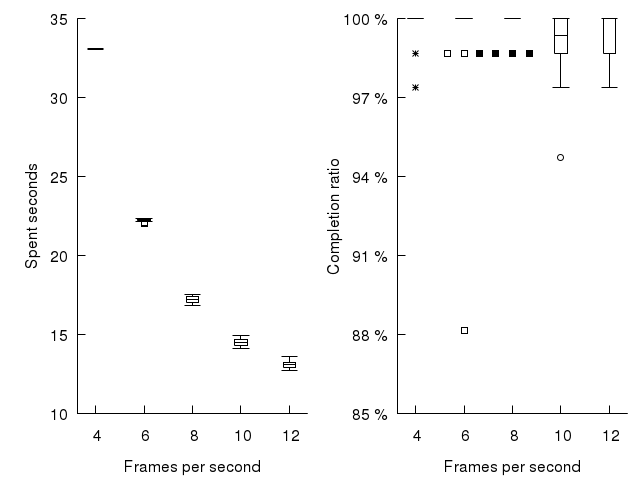
\includegraphics[width=\linewidth]{stream.png}
\caption{Time to send data in Stream mode}
\label{img-expstream}
\end{center}
\end{figure}

\subsubsection{Paper Swiping}\label{subsub:swipe}

The ability to send streams of data in Lake mode can also be used to supplement QR codes' inherently limited capacity. When displaying a printed code on a piece of paper, large amounts of data can be carried only through increasing the code's resolution; however, resolution can only be increased up to a certain, predefined limit.\footnote{4,296 alpha-numeric characters, or 3,222 bytes assuming Base-64 encoding.} Moreover, for higher resolutions, the code may become hard to read using entry-level, low-resolution cameras. Therefore, it is safe to assume that, using existing QR code technology, no more than 3,000 bytes of data can be transferred using a QR code.

This limitation can be overcome by the use of the BufferTannen protocol. Although no code larger than roughly 4,000 bytes can be created, multiple such codes can be lined on a piece of paper. Each such code can be formatted to contain a single frame of data sent by the BufferTannen protocol in Lake Mode. It suffices for a user to swipe the camera over these multiple codes; by virtue of Lake Mode, the order in which the codes are scanned is irrelevant, and the complete piece of data can be correctly reconstructed from the individual frames. It is therefore possible to transmit theoretically unlimited amounts of data, while using codes of a lower resolution (this lower resolution being compensated by the presence of more than one code).

To verify this claim, we printed on a piece of paper the contents of a 37 kb file as a sequence of QR codes, processed as frames through BufferTannen in Lake Mode. We then hovered the camera over that sheet of paper at arm's length (see Figure \ref{fig:qr:paper-swipe}). The software's user interface displayed in real time the number of frames remaining to be decoded and their location in the complete stream, giving indications to the user as to which codes to swipe over. It shall be noted that the camera operated in ``film'' mode, and not in ``snapshot'' mode. In other words, images were continuously captured by the camera as it was being moved over the sheet; the user did not need to point and click at each individual QR code (which would be fastidious).

\begin{figure}
\centering
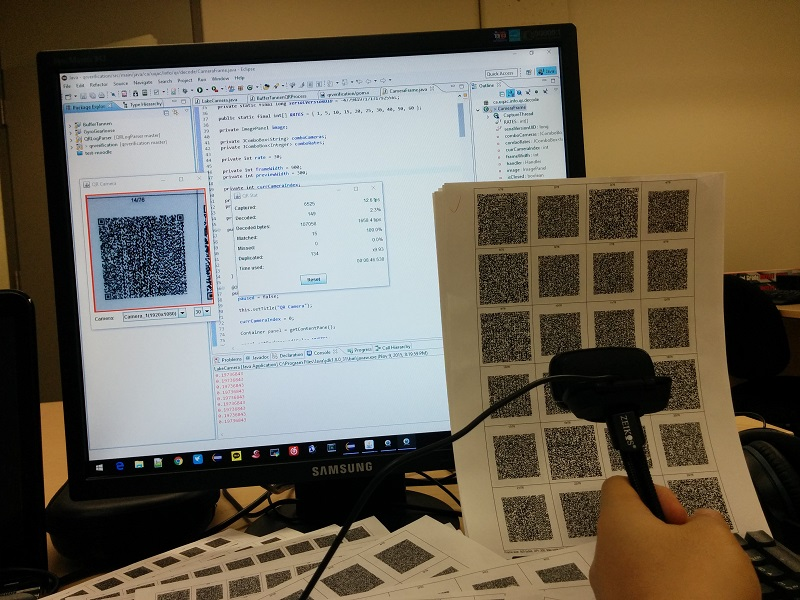
\includegraphics[width=\linewidth]{swipe.jpg}
\caption{Swiping the camera over a set of QR codes to reconstruct the contents of a larger file.}
\label{fig:qr:paper-swipe}
\end{figure}

The error correction level chosen was L and the sizes of raw data per code that we tested were 500, 750, 1,000, 1,250, 1,500, 1,750, and 2,000 bytes. With 500 bytes there were 76 codes while with 2,000 bytes there were only 19. After being encapsulated by BufferTannen protocol, the final sizes of data used to generate the QR codes became correspondingly 723, 1,055, 1,391, 1,724, 2,054, 2,389, and 2,722 bytes. The codes were printed at 300 dpi and 600 dpi on standard office paper, and we programmed to give each edge of every code 500 dots in the paper.

At 300 dpi, the codes of size ranging from 500 to 1,250 bytes were all decoded successfully and smoothly. However, when the size reaches 1,500 bytes, the decoding becomes more problematic. For some codes, we had to retry for several times by sticking the camera near the paper for a few seconds, yet among the total 31 codes, three remained impossible to decode at all. In the case of codes of 1,750 and 2,000 bytes, none of the codes could be decoded. This can be explained by the fact that higher density codes entail that each module of the code is smaller and hence harder to capture. For example, the edge of a 500-bytes and L-level code is about 77 modules, so each module can have approximately 6 dots in the paper, while the edge of a 2000-bytes, L-level code is 149 modules, so each module amounts to only 3 printed dots.

At 600 dpi, none of the codes could be decoded, no matter how many bytes they carried. The reason is that the codes printed at 600 dpi are too small and the camera has to approach very closely to the paper, but the captured images were all blurred and out of focus. It therefore seems that codes printed at 600 dpi are beyond the ability of a standard web camera.

Nevertheless, this experiment demonstrates the viability of the concept of hovering a camera across an array of QR codes. Our empirical findings indicate that a stream of data can be split into a set of QR codes of about 1,000 bytes each, the contents of which correspond to individual frames of the BufferTannen protocol containing the data to be transmitted. Swiping the camera over this set of codes, in no particular order, is sufficient to reconstruct on the device side the complete data contents.

%% }}} --- Section

%% -----------------------
%% Section: Conclusion
%% -----------------------
\section{Conclusion}\label{sec:qr:conclusion} %% {{{

In this chapter, we presented a solution for an one-way communication channel based on QR codes, and performed experiments to measure its performance. We first experimentally tested the characteristics of a QR data stream under various conditions, and extracted the parameters maximizing the effective bandwidth of the channel. However, since that channel is inherently error-prone and low-bandwidth, we then introduced BufferTannen, a protocol designed especially for this kind of channel. BufferTannen takes care of splitting, marshaling, and to some extend compressing the data to transmit in order to maximize the efficiency of the QR code stream. The feasibility of this approach was then empirically observed through a new set of experiments.

Within the limits of the protocol and of the communication channel, the presented results can be put to good use in a variety of situations. In limited environments where the use of radio signal or cables is forbidden or difficult, our approach can provide an easy way to communicate between peers, either as an emergency backup or as a primary means. Furthermore, the evolution of the quality of both display and image capture devices makes it possible to foresee increased transmission rates in the future. %as the performance of common devices keeps increasing, the symbols containing more data, or even some more complicated symbol formats can be brought into concern.
Finally, the aforementioned techniques could be turned into a bidirectional communication link in the case of endpoints equipped with both a camera and a display. In such a case, acknowledgments of correctly decoded images could be exchanged, which in turn would allow resending data on demand and increase the effective bandwidth.

%% }}} --- Section